% Created 2019-09-27 Fri 12:29
% Intended LaTeX compiler: pdflatex
\documentclass[11pt]{article}
\usepackage[utf8]{inputenc}
\usepackage[T1]{fontenc}
\usepackage{graphicx}
\usepackage{grffile}
\usepackage{longtable}
\usepackage{wrapfig}
\usepackage{rotating}
\usepackage[normalem]{ulem}
\usepackage{amsmath}
\usepackage{textcomp}
\usepackage{amssymb}
\usepackage{capt-of}
\usepackage{hyperref}
\author{Ivan Nikolic}
\date{\today}
\title{}
\hypersetup{
 pdfauthor={Ivan Nikolic},
 pdftitle={},
 pdfkeywords={},
 pdfsubject={},
 pdfcreator={Emacs 26.2 (Org mode 9.1.9)}, 
 pdflang={English}}
\begin{document}

\tableofcontents


\section{Samples}
\label{sec:orga3746e5}

\begin{center}
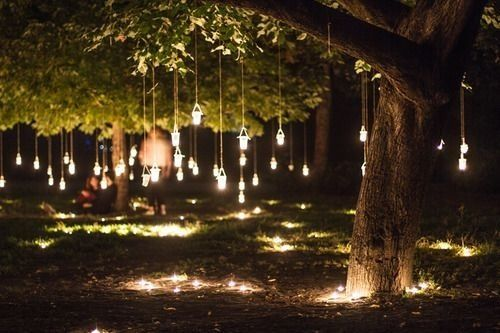
\includegraphics[width=.9\linewidth]{./samples/3.jpg}
\end{center}
\begin{center}
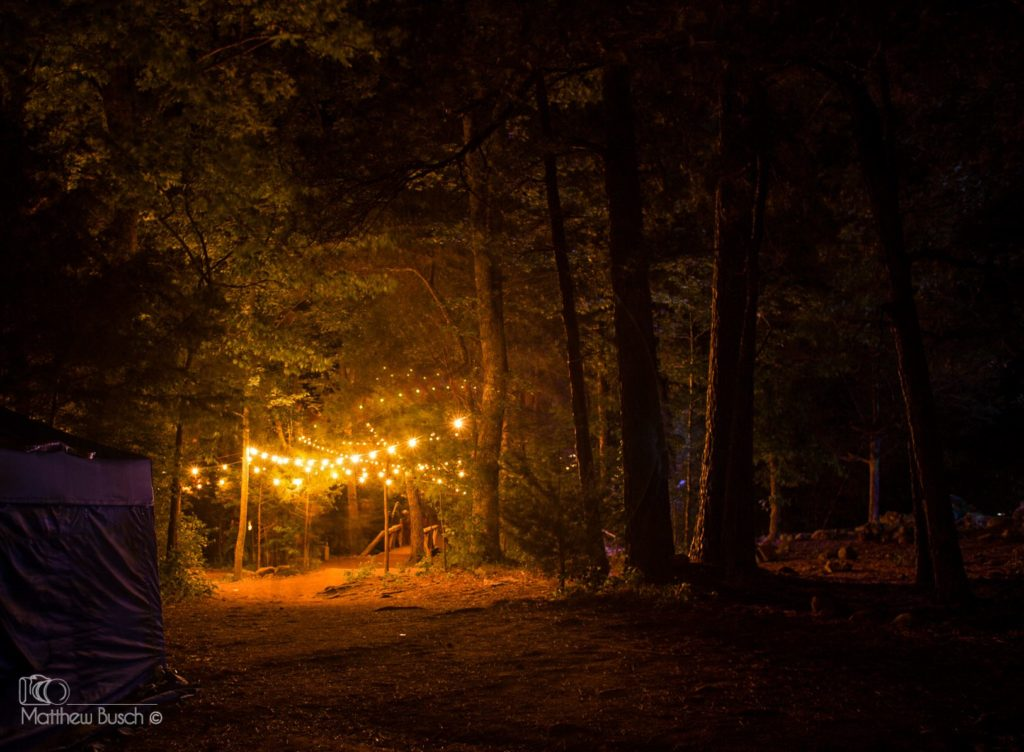
\includegraphics[width=.9\linewidth]{./samples/4.jpg}
\end{center}
\begin{center}
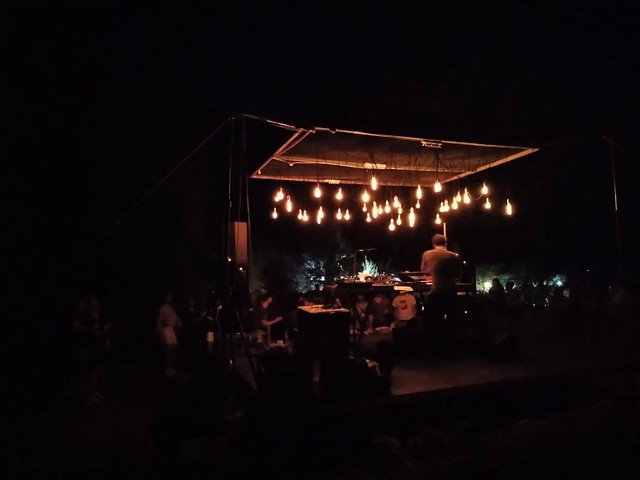
\includegraphics[width=.9\linewidth]{./samples/5.jpg}
\end{center}
\begin{center}
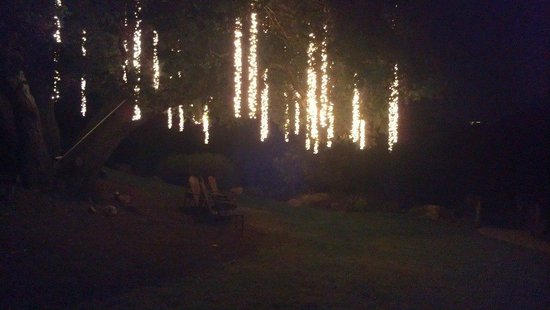
\includegraphics[width=.9\linewidth]{./samples/1.jpg}
\end{center}

\section{generative "Biologically inspired" diffusers}
\label{sec:org864840c}

\url{https://www.thingiverse.com/thing:1883446}

for diffusers: 

\begin{center}
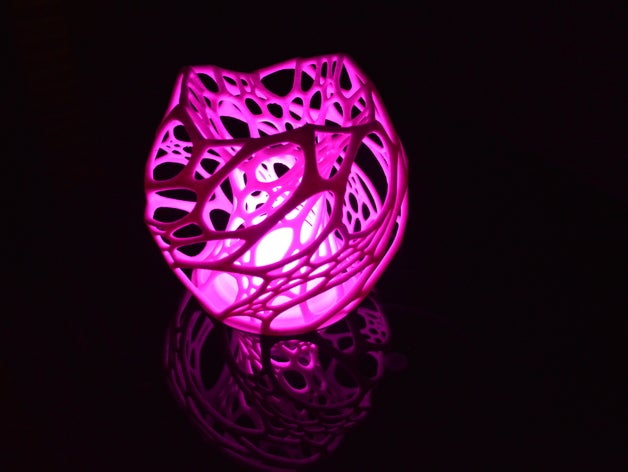
\includegraphics[width=.9\linewidth]{./samples/bulb1.jpg}
\end{center}
\begin{center}
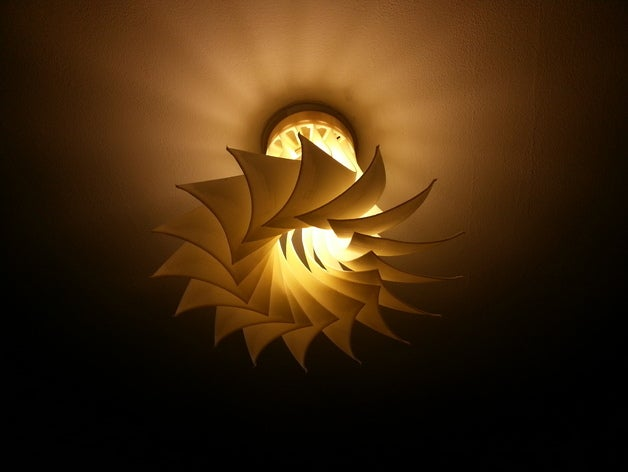
\includegraphics[width=.9\linewidth]{./samples/bulb3.jpg}
\end{center}
\begin{center}
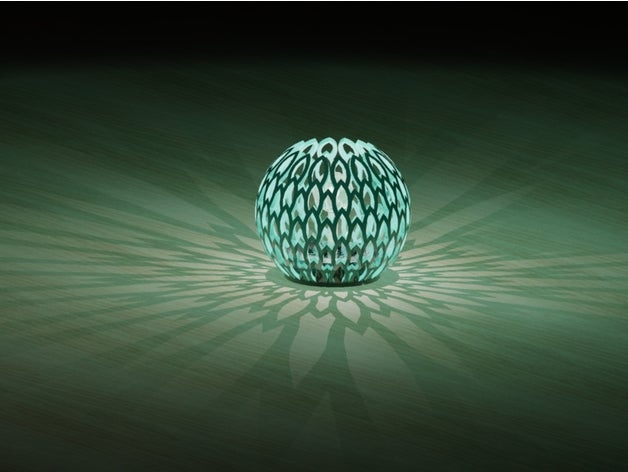
\includegraphics[width=.9\linewidth]{./samples/bulb4.jpg}
\end{center}

every component can be made in a similar style

\section{Tech Structure}
\label{sec:org053d793}

\begin{center}

\includegraphics[width=.9\linewidth]{basic.png}
\end{center}

\section{ESP based mesh control network}
\label{sec:org009a833}
\url{https://github.com/gmag11/painlessMesh}

\url{https://github.com/Coopdis/easyMesh}

\url{https://github.com/martin-ger/esp\_wifi\_repeater}

let's use lua, write a module dude

\section{Expected power draw}
\label{sec:org23b5303}
WS2812B - \url{https://www.seeedstudio.com/document/pdf/WS2812B\%20Datasheet.pdf}

1 LED draws max 5 mA from a 5V supply (tested)

9 leds per bulb = \textasciitilde{}50ma max

\subsection{{\bfseries\sffamily TODO} test with covers to make sure 9 led bulb is bright enough}
\label{sec:orga3a1a03}


\section{Battery}
\label{sec:orgaace87d}
3200 mah seems ok,
3 18650 cells in 3S1P configuration to get 9.6v - 12.6v

Battery cell 3 EUR - full bat is 9 EUR

roughly,

\begin{center}
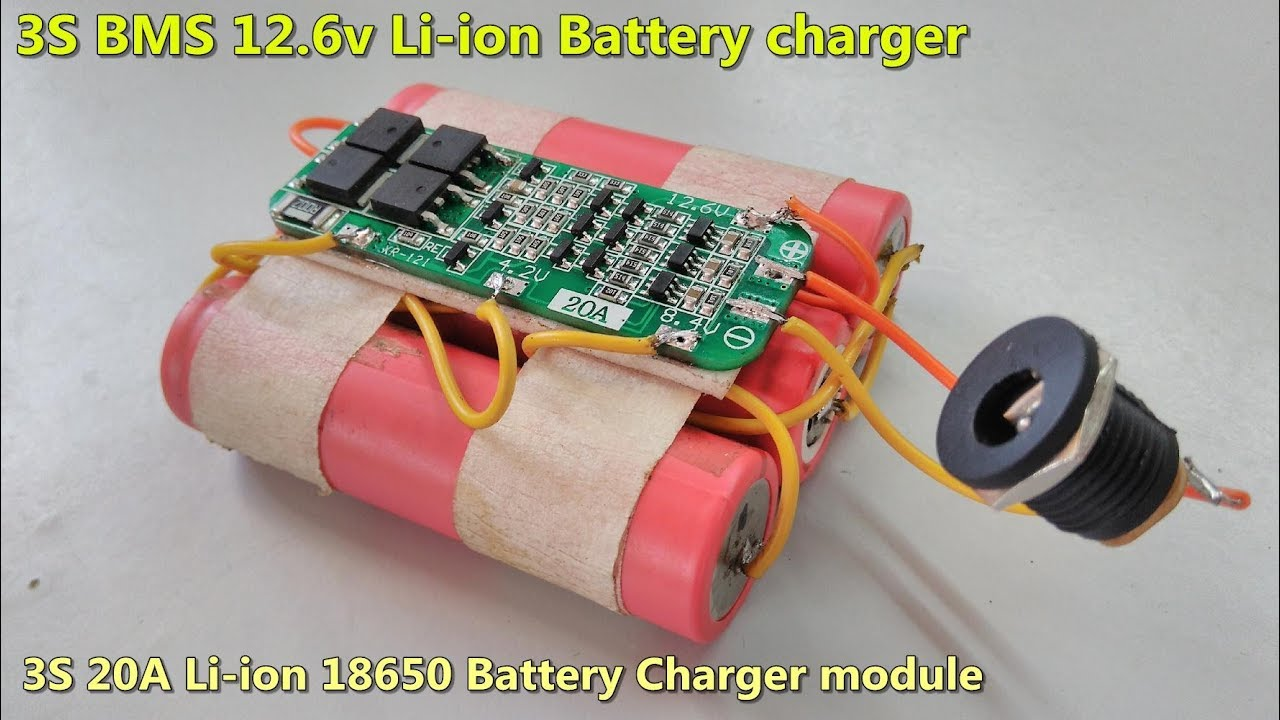
\includegraphics[width=.9\linewidth]{./samples/battery.jpg}
\end{center}

\section{Solar panel}
\label{sec:orgacfab00}
Solar panel \textasciitilde{}10W seems ok

\section{Estimates}
\label{sec:org76c40c6}

\begin{center}
\begin{tabular}{rrrrrrrr}
mA/LED & LED/Bulb & Bulbs & Battery (mAh) & Solar (mA) & Total Draw (mA) & Working Hours & Charging Hours\\
\hline
5 & 9 & 6 & 3200 & 10000 & 270.0 & 12 & 5\\
5 & 9 & 12 & 3200 & 10000 & 540.0 & 6 & 5\\
5 & 12 & 6 & 3200 & 10000 & 360.0 & 9 & 5\\
5 & 15 & 6 & 3200 & 10000 & 450.0 & 7 & 5\\
\end{tabular}
\end{center}


\section{modular and interchangable connectors}
\label{sec:org3ab14e8}
check GX16 standard,

\begin{center}
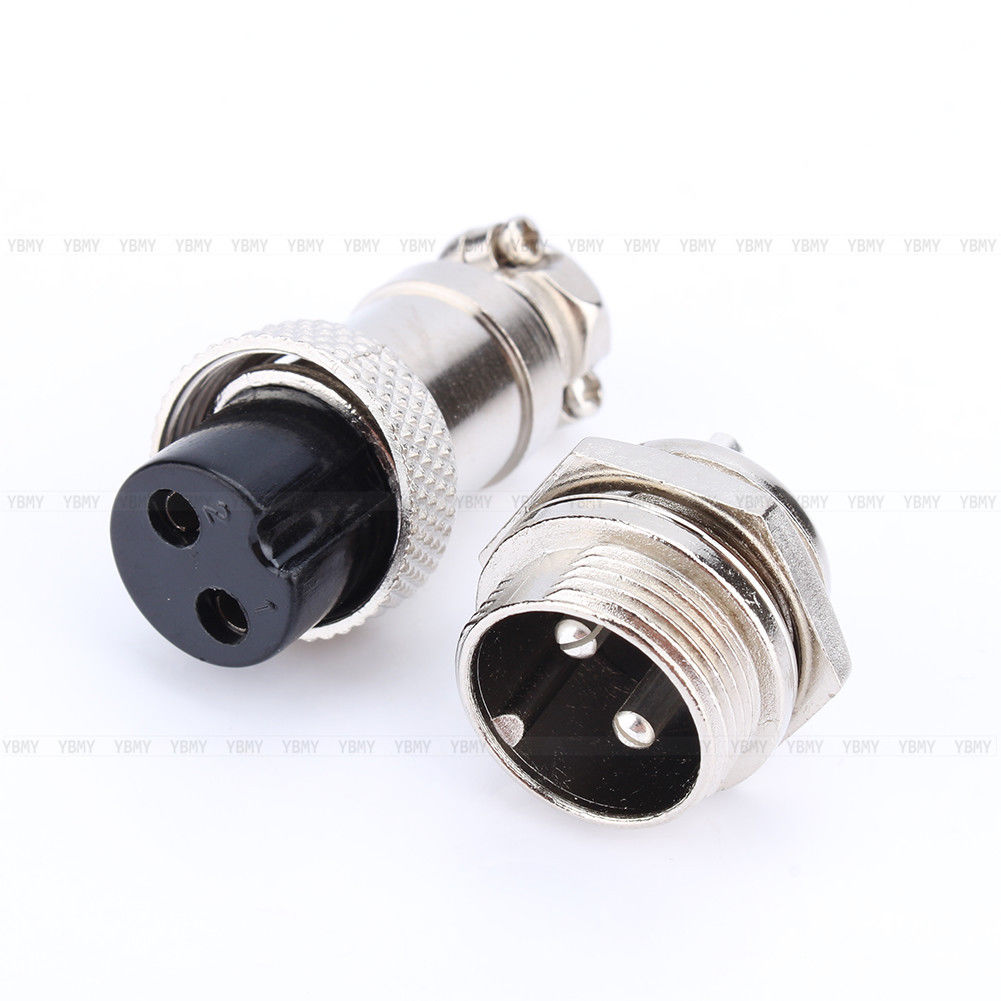
\includegraphics[width=.9\linewidth]{./samples/powerconnector1.jpg}
\end{center}

\begin{itemize}
\item both solar and battery have standard input/output connectors, so they can be chained, or replaced with a grid/centralized source
\item dark outside? chain some solar panels
\item need more capaciy? chain batteries
\item running on the grid? get rid of solar and batteries, connect grid directly
\end{itemize}

\begin{center}

\includegraphics[width=.9\linewidth]{simple1.png}
\end{center}

think about flexibility on numbers of bulbs with some top limit (12?) (autodetect strip length?)

GX16 for bulbs as well (6 pin)?
  \begin{center}
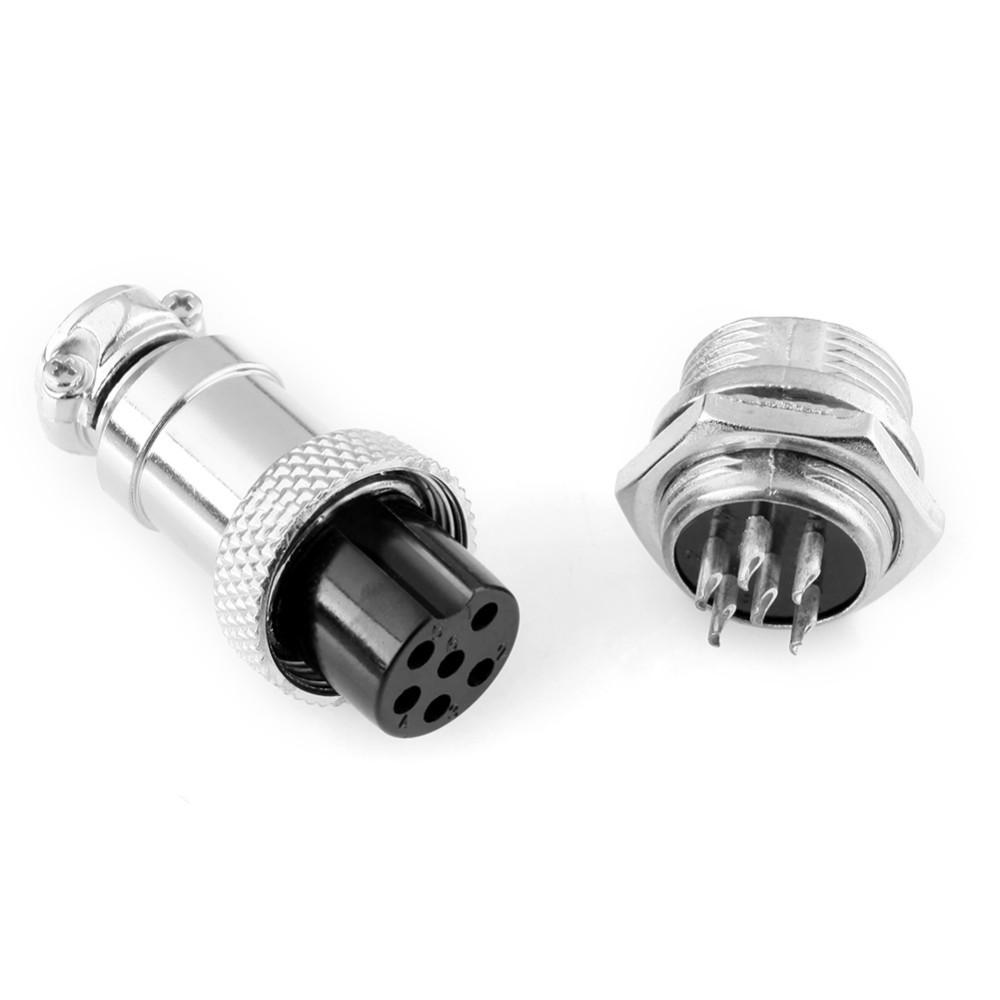
\includegraphics[width=.9\linewidth]{./samples/bulbconnector1.jpg}
\end{center}

\begin{itemize}
\item since we are running on a bus, it' possible to drag one cable far and then split it into multiple cables for multiple bulbs wih some Y or X connectors

\item maybe controller has only one connector, we use spliters to distribute
\end{itemize}


\begin{center}

\includegraphics[width=.9\linewidth]{splitter.png}
\end{center}



\section{Software}
\label{sec:org36218a2}
\begin{itemize}
\item 3d position map of bulbs for running spacial algorithms
\item explore possibility of automatically triangulating control nodes based on signal strength
\item system wide battery monitoring via voltage measuring on controllers
\end{itemize}
\end{document}
